\documentclass[a4paper, 14pt]{article}
\usepackage[pdftex,
    pdfauthor={Егоров Геннадий Викторович},
    pdftitle={Сбоник лекций по курсу радиационнной физики для 4 курса Медицинской физики},
    pdfsubject={Радиационная физика},
    pdfkeywords={Ионизирующее излучение, Дозиметрия, Радиоактивность, Ремизов, 4 курс Медицинская физика},
    pdfproducer={LuaLatex with hyperref},
    pdfcreator={Lualatex}
]{hyperref}
\usepackage{latexsym,amsmath,amssymb,amsbsy,graphicx}
\usepackage{icomma}
\usepackage{graphicx}
\graphicspath{{images/}}
\DeclareGraphicsExtensions{.pdf,.png,.jpg}
%%%%%%%%%%%%%%%%%%%%%%%%Оформление по ГОСТу
\usepackage{fontspec}
\setmainfont{Times New Roman}
\usepackage[russian, english]{babel} %Поддержка русского языка
\usepackage[14pt]{extsizes} % для того чтобы задать нестандартный 14-ый размер шрифта
\usepackage{indentfirst} %Задаёт отступ самого первого абзаца
\setlength\parindent{1.25cm}
\usepackage[a4paper, left=3cm, top=1.5cm, right=1.5cm, bottom=2cm]{geometry}
\usepackage{setspace}
\sloppy %Выравнивание текст по ширине
\onehalfspacing %Полуторный интервал
\title{Лекции по радиационной физике}
\author{Егоров Г.В.}
\date{\selectlanguage{russian}\today}
\begin{document}
\maketitle
\section{Предмет и метод радиационной биофизики. Актуальность исследования
биологического действия ионизирующего излучения. Разделы радиобиологии}
\textbf{Радиационная биофизика}~---~это наука, изучающая молекулярные механизмы
биологического действия ионизирующего и неионизирующего излучения на органы,
вычисляющие последовательную картину изменений, начиная от поглощенной
энергии радиации отдельных молекул до сложных биологических изменений в клетке
и органе.

Радиационная биофизика изучает радиобиологические проблемы с позиции
биофизики. Если радиобиология изучает влияние излучения на биологические
объекты, то биофизика изучает молекулярные взаимодействия, лежащие в основе
нормальных и патологических жизненных явлений.

\textbf{Ионизирующим излучением} (проникающей радиацией) называют
высокочастотные электромагнитные излучения энергетических фотонов, которые
превышает величину потенциала ионизации больше, чем 10 эВ. К ионизирующему
излучению относятся рентгеновское излучение и гамма-излучение.
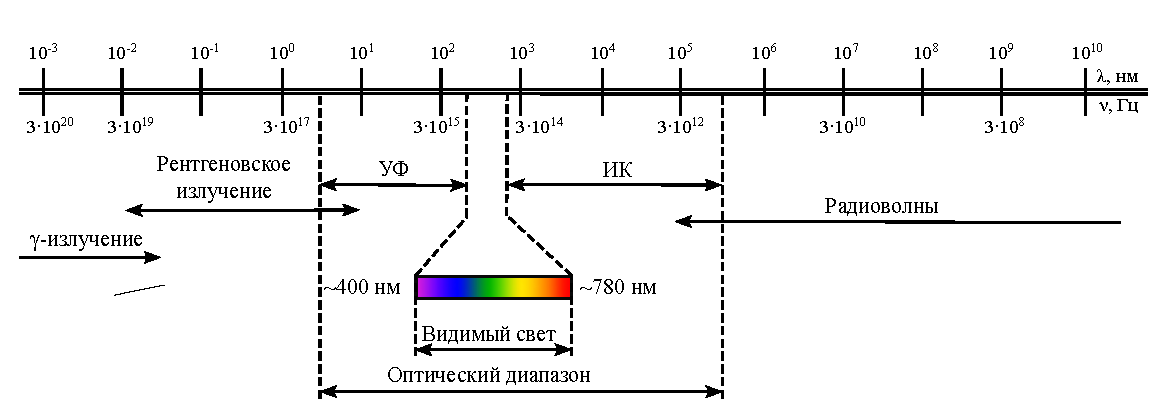
\includegraphics[width=\textwidth]{EMW}
\[ E = h\nu \frac{hc}{\gamma}, 1\;\text{эВ} = 1,6 \cdot 10^{-19}\;\text{Дж}\]
\[ E = 10\;\text{эВ} = 1,6 \cdot 10^{-18}\;\text{Дж}\]
\[ \gamma \frac{hc}{E} = \frac{6,6\cdot 10^{-34} \cdot 3 \cdot 10^8}{1,6 \cdot 10^{-19}} = 1,2 \cdot 10^{-7}\;\text{м} = 120\;\text{нм}\]
Рентгеновское излучение и гамма-излучение отличаются по энергии, длине
волны и по происхождению.

Рентгеновское излучение делится на \textit{тормозное} и \textit{характеристическое}.

\textbf{Тормозное} возникает при торможении заряженных частиц при большом
ускорении. Энергетический спектр является непрерывным.

\textbf{Характеристическое} возникает при переходах между далеко расположенными
энергетическими уровнями. Спектр излучения дискретный.

Гамма-излучение возникает либо при ядерных реакциях, либо при переходах в
энергетических уровнях в ядрах.

\textbf{Оптические излучения} не способны к ионизации молекул, лишены высокой
проникающей способности.
К ионизирующему излучение также относятся: корпускулярные излучения, а именно: $\beta$-частицы, т.е. электроны, позитроны, протоны, $\alpha$-частицы, так же нейтроны и др. частицы.

Актуальность исследования биологического действия ионизирующего излучения:
\begin{enumerate}
    \item Все живое постоянно подвергается воздействию постоянного естественного
    радиационного фона;
    \begin{itemize}
        \item космическая радиация;
        \item излучение радиоактивных элементов, залегающих в поверхностных слоях
        земной коры и входящих в состав живых организмов и продуктов питания;
    \end{itemize}
    \item В связи с техногенной деятельностью человека (взрывы, аварии)
    радиационный фон во многих регионах значительно выше естественного, поэтому
    возникает необходимость исследования влияния этого повышенного фона на здоровье
    и жизнь человека;
    \item Ионизирующее излучение используется как диагностическое и
    терапевтическое средство при многочисленных заболеваниях
\end{enumerate}
Радиационная терапия основана на изучении механизмов взаимодействия
излучения с веществом.

\textbf{Радиобиология}~--~это комплексная наука, в которой развиваются многие
направления:
\begin{enumerate}
    \item Радиационная экология и генетика
    \item Радиационная биохимия и цитология
    \item Радиационная медицина и генетика
    \item Радиационная биофизика
\end{enumerate}

\textbf{Радиационная биофизика} занимает особое место в радиобиологии. Она
выясняет физико-химические и молекулярные механизмы первичных процессов
лучевых изменений, протекающих с момента возникновения ионизирующего
возбуждения атомов и молекул до появления видимых структурных и функциональных изменений.

Для решения этой задачи необходимо углубленный анализ процессов,
проходимых после поглощения энергии квантов в живой системе, описание всех
этапов в терминах молекулярных изменений и создание единой картины, отражающей
всю последовательность реакций, приводящих в зависимости величины дозы к
лучевым изменениям или поражениям.

\section{История развития радиационной биофизики}
Радиобиология возникла после открытия рентгеновского излучения, которое
произошло в конце 19 веке.

В декабре 1895г., Рентгеном был сделан первый рентгеновский снимок кисти своей руки. Результаты работы были изложены в рукописи об открытии катодных проникающих Х-лучей.

В январе 1896 г. брошюра Рентгена «Новый род лучей» вышла в свет на
нескольких языках, открытие стало достоянием мировой общественности.

Март 1996, Анри Беккерель обнаружил явление~---~самопроизвольное испускание
невидимых глазу проникающих излучений ($\alpha, \beta$ и $\gamma$), исходящих от солей урана.

Через два года Мария и Пьер Кюри выделили из урановой смолы ранее не
известные элементы, так же, подобно урану, испускающие излучения, которым они
дали название радий и полоний. Для явления, свойственного этим, а в последующем
другим подобным элементам был предложен термин \textbf{радиоактивность}.

Открытие урановых, а затем и ториевых лучей послужило началом
исследований \textit{естественной (природной) радиоактивности}.

1934г. Ирен Кюри и Фридерих Жулио Кюри открыли новое явление~---~искусственную радиоактивности (при исследовании ядерной реакции $^{27}Аl(\alpha,n)^{30}P$ %TODO: Нужно уточнить реакцию
обнаружили образование нового, не встречающегося ранее в природе радионуклида~---~фосфора $^{30}Р$).

\subsection{Развитие радиобиологии}
Петербуржский физиолог Тарханов провел исследование на лягушках и
насекомых и пришел к выводу, что Х-лучами можно не только фотографировать, но и
влиять на ход жизненных функций.

Ефим Лондон в 1896 году начал исследование по экспериментальной
радиобиологии.

Первая официальная информация о патологическом влиянии радиации была
опубликована в 1901 году, которая сообщила, что радий вызывает ожоги кожи.

\textbf{Важными задачами} радиобиологии в то время была необходимость точной и
количественной оценки дозы радиации, вначале появились условные единицы
биологических доз.

% HED (кожная-эритемная доза) %TODO: Зачем это здесь?
В 1901 и последующие годы появилось множество работ о лучевом поражении
кожи. В 1902 году описан первый случай лучевого рака кожи. Выяснилось, что
возникающая радиация не только воздействует на кожу, но и вызывает лучевое
поражение внутренних органов и тканей, а также гибель живых организмов и
человека. Опыты Лондона в России и Хейкеля в Германии.

В Последующие годы выяснились сведения о высокой биологической эффективности нового вида излучений стимулировало мощный взрыв радиобиологических работ, характеризующий \textbf{начальный, описательный период} в истории радиобиологии.  

\subsection{Открытие закона радиочувствительности клеток}
В 1906 г. французские радиобиологи Жан Бергонье и Луи Трибондо сформулировали фундаментальный \textbf{закон (правило) радиочувствительности клеток:} \textit{ионизирующее излучение оказывает тем большее повреждающее действие на клетки, чем интенсивнее те делятся и чем менее определенно выражены их морфология и функция, т. е. чем менее они дифференцированны}. 

По мере накопления фактов становилось ясным, что ионизирующие излучения, в зависимости от интенсивности источника радиации и длительности облучения, способны вызывать повреждения и гибель любого биологического объекта, любой биологической системы.

Начиная с 1910 г. М. И. Неменов и сотрудники публикуют работы по
выяснению изменений обмена веществ при лучевом поражении и о сходстве лучевых
изменений с процессами патологии раннего старения.
\end{document}